\documentclass[11pt, letterpaper, includehead]{article}

%%%%%%%%%%%%%%%%%%%%% Pre-document %%%%%%%%%%%%%%%%%%%%%
\usepackage{fancyhdr}  % Allow for headers
\usepackage{graphicx}  % Allow for figures 
\usepackage{float}     % Allow for figure inserted in specified location
\usepackage{amsmath}   % Allow for aligned math
\usepackage{array}     % Allow for cell width manipulatio
\usepackage{nicematrix}
\usepackage{amssymb} % Uhhhh what was this????

\setlength{\parindent}{0pt} % Remove auto paragraph indents

% Get rid of those big ass margins
\usepackage[margin=1in]{geometry}

% Table cell formatting
\setlength{\arrayrulewidth}{0.25mm}
\setlength{\tabcolsep}{11pt}
\renewcommand{\arraystretch}{1.2}

\begin{document}

%%%%%%%%%%%%%%%%%%%%% Title Page %%%%%%%%%%%%%%%%%%%%%
\begin{titlepage}
  \begin{center}
    \Huge{\textbf{Lab 3}}\\
    \Huge{Vectors}
    \vfill
    \begin{figure}[H] % H makes the figure insert at the position in the document
      \centering 
      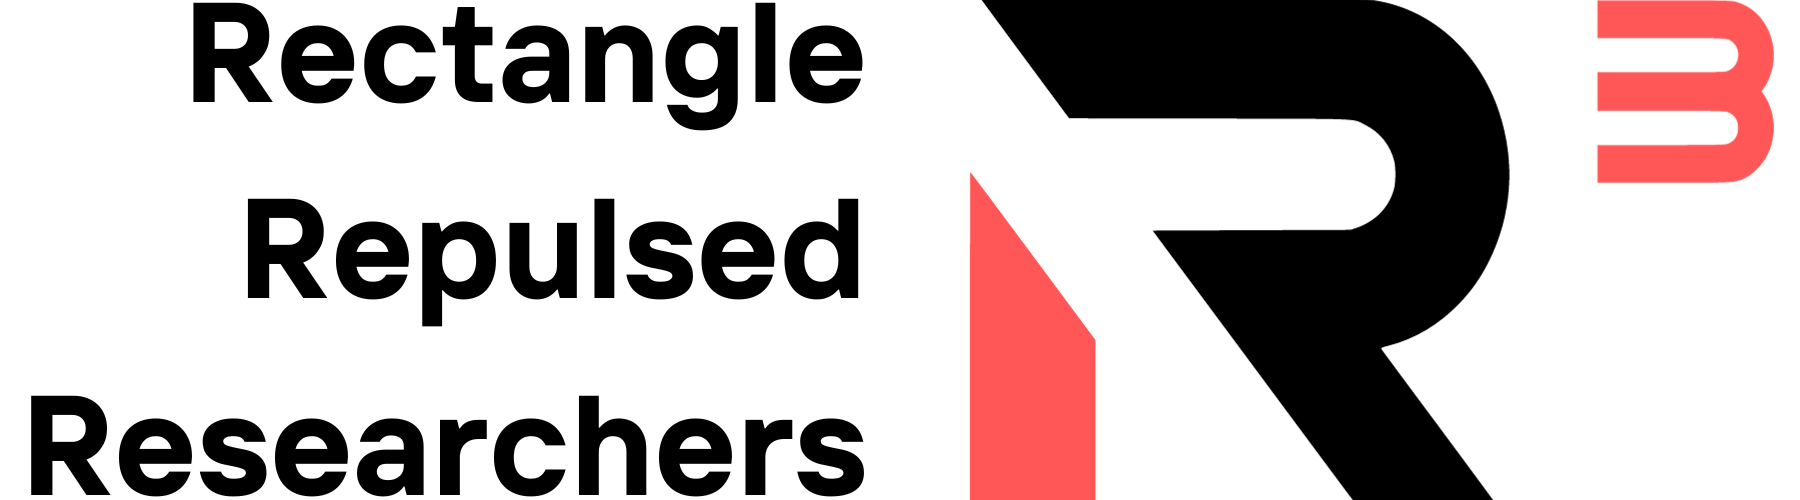
\includegraphics[width=6cm]{../logo.png}
    \end{figure}
    \large{\textbf{Rectangle Repulsed Researchers}}\\
    \large{Julian Barossi, Liam Gilligan, Stephanie L'Heureux}\\
    \vspace{0.5cm}
    \normalsize
    \today
  \end{center}
\end{titlepage}

%%%%%%%%%%%%%%%%%%%%% TABLE OF CONTENTS %%%%%%%%%%%%%%%%%%%%%
\tableofcontents
\pagebreak % Move to next page

% Add a nice fancy header
\pagestyle{fancy}
\fancyhead{}
\fancyhead[C]{\textbf{Lab 3:} Vectors}

\section{Measuring the Time of a Dropped Pencil} % 1

\subsection{Predicted time $t_{thy}$} % 1.1
The calculations below predict the time ($t_{thy}$) for the pencil to
fall from rest a distance of $2.0m$.

$$y       = y_0 + v_{y_0}t + \frac{1}{2}a_yt^2$$
$$-y_0    = \frac{1}{2}a_yt^2$$
$$t       = \sqrt{\frac{-2y_0}{a_y}}$$
$$t       = \sqrt{\frac{-2(2.0m)}{-9.8m/s^2}}$$
$${t_{thy} = 0.6388765...s \Rightarrow  \boxed{0.64s}}$$

\subsection{Recorded time} % 1.2 
\begin{center}
  \begin{tabular}[H]{| m{2cm} | m{2cm} |}
    \hline
    \textbf{Trial} & \textbf{Time (s)} \\
    \hline
    1              & 0.55              \\
    \hline
    2              & 0.69              \\
    \hline
    3              & 0.69              \\
    \hline
    4              & 0.65              \\
    \hline
    5              & 0.67              \\
    \hline
    6              & 0.58              \\
    \hline
    7              & 0.61              \\
    \hline
    8              & 0.64              \\
    \hline
    9              & 0.63              \\
    \hline
    10             & 0.68              \\
    \hline
    11             & 0.61              \\
    \hline
    12             & 0.63              \\
    \hline
    13             & 0.67              \\
    \hline
    14             & 0.64              \\
    \hline
    15             & 0.65              \\
    \hline
    16             & 0.68              \\
    \hline
    17             & 0.66              \\
    \hline
    18             & 0.66              \\
    \hline
    19             & 0.56              \\
    \hline
    20             & 0.66              \\
    \hline
  \end{tabular}
\end{center}

\setcounter{subsection}{3} % Make next section start at 1.4
\subsection{Mean average time for 100 measurements} % 1.4
Data collected by physical instruments always includes some degree
of error. Error in this context does not necessarily mean a mistake,
but rather an unavoidable uncertainty due to random fluctuations in
measurement tools or statistical factors. This type of error is
defined as a random error. If multiple measurements of a quantity
are taken, by random error, sometimes the measurement will overestimate
the data, and just as likely the result may be an underestimate. A
typical result with minimal random error may be found by taking the
mean ($\bar{t}$) of repeated experiments.

\begin{center}
  \begin{tabular}{|   m{2cm}  |  m{2cm}  |  m{2cm}  |  m{2cm}  |  m{2cm}  |  m{2cm}  | }
    \hline
    \multicolumn{5}{|c|}{\textbf{Time (s)}}\\
    \hline
    \textbf{Kate} & \textbf{Jesus} & \textbf{Sam} & \textbf{Stephanie} & \textbf{Liam} \\
    \hline
    0.67          & 0.53           & 0.68         & 0.55               & 0.66          \\
    \hline
    0.57          & 0.66           & 0.71         & 0.69               & 0.68          \\
    \hline
    0.51          & 0.61           & 0.64         & 0.69               & 0.66          \\
    \hline
    0.56          & 0.52           & 0.61         & 0.65               & 0.60          \\
    \hline
    0.55          & 0.61           & 0.63         & 0.67               & 0.55          \\
    \hline
    0.59          & 0.63           & 0.70         & 0.58               & 0.55          \\
    \hline
    0.63          & 0.61           & 0.64         & 0.61               & 0.60          \\
    \hline
    0.63          & 0.64           & 0.72         & 0.64               & 0.56          \\
    \hline
    0.63          & 0.67           & 0.65         & 0.63               & 0.61          \\
    \hline
    0.76          & 0.69           & 0.62         & 0.68               & 0.63          \\
    \hline
    0.56          & 0.53           & 0.61         & 0.61               & 0.66          \\
    \hline
    0.70          & 0.56           & 0.60         & 0.63               & 0.68          \\
    \hline
    0.66          & 0.59           & 0.64         & 0.67               & 0.68          \\
    \hline
    0.74          & 0.54           & 0.62         & 0.64               & 0.70          \\
    \hline
    0.67          & 0.64           & 0.66         & 0.65               & 0.63          \\
    \hline
    0.71          & 0.61           & 0.67         & 0.68               & 0.63          \\
    \hline
    0.75          & 0.57           & 0.65         & 0.66               & 0.65          \\
    \hline
    0.58          & 0.63           & 0.59         & 0.66               & 0.70          \\
    \hline
    0.70          & 0.56           & 0.64         & 0.56               & 0.61          \\
    \hline
    0.60          & 0.64           & 0.64         & 0.66               & 0.60          \\
    \hline
    \hline
    \multicolumn{5}{|c|}{\textbf{Average ($\bar{t}$ for each person) (s)}} \\
    \hline
    0.639         & 0.602          & 0.646        & 0.641              & 0.632         \\
    \hline
  \end{tabular}
\end{center}
$$\bar{t} = \frac{1}{n}\sum t_i = \frac{t_1 + t_2 + t_3 + ... + t_n}{n}$$
$$\bar{t}_{total} = 0.6318...s \Rightarrow \boxed{0.63s}$$

\subsection{Standard deviation for 100 measurements} % 1.5
The mean found in the previous section gives the best representative
value of a set. However, this measurement neglects significant
information regarding the original data. The mean alone fails to
express how dispersed the data points are. A set of values may be
concentrated, scattered, or evenly dispersed and from just the mean it is impossible to discern.
For this reason, it is advised to also provide the standard deviation
when presenting results. The standard deviation conveys the variability in a set.
$$\sigma = \sqrt{\frac{1}{N - 1}\sum_{i = 1}^{N} (d_i)^2} = \sqrt{\frac{1}{N - 1}\sum_{i = 1}^{N} (t_i - \bar{t})^2}$$\\
$$\sigma = \sqrt{\frac{1}{100 - 1}\sum_{i = 1}^{100}(t_i - 0.6318s)^2} = 0.05224998188...s \Rightarrow \boxed{0.052s}$$


\subsection{Values within one standard deviation} % 1.6 
Approximately $68\%$ of the values of any measurement should fall within one
standard deviation ($1 \sigma$) of the mean value ($\bar{t}$). Therefore $68\%$ of measured
values should be $\geq (\bar{t} - \sigma_t)$ and $\leq (\bar{t} + \sigma_t)$\\

\subsubsection{Percentage of values which fall in one standard deviation} %1.6.1
$$\frac{\# measurements \in [\bar{t} - \sigma_t, \bar{t} + \sigma_t]}{N} \\$$
$$\frac{\# measurements \in [0.631s - 0.0522s, 0.631s + 0.0522s]}{100} \\$$
$$\frac{\# measurements \in [0.5788s, 0.6832s]}{100} \\$$
% $$\frac{68}{100}$$
$$\boxed{69\%}$$

\subsubsection{Does the data match the statistical prediction} %1.6.2
If the collected data represents a normal distribution,
the dispersal of data points and the standard deviation relate such that the mean is
$\geq (\bar{t} - 2\sigma_t)$ and $\leq (\bar{t} + 2\sigma_t)$ according
to statistical theory. The calculations in the section above show that
for our data set, statistical theory nearly matches the actual data.
$69\%$ percent of the data falls within one standard deviation of the mean.

\subsection{Values within two standard deviations} % 1.7
Approximately $95\%$ of the values of any measurement should fall within two
standard deviations ($2 \sigma$) of the mean value ($\bar{t}$). Therefore $95\%$ of measured
values should be $\geq (t - 2 \sigma_t)$ and $\leq (t + 2 \sigma_t)$

\subsubsection{Percentage of values which fall in two standard deviations} % 1.7.1
$$\frac{\# measurements \in [\bar{t} - 2\sigma_t, \bar{t} + 2\sigma_t]}{N} \\$$
$$\frac{\# measurements \in [0.631s - 2(0.0522s), 0.631s + 2(0.0522s)]}{100} \\$$
$$\frac{\# measurements \in [0.5266s, 0.7354s]}{100}$$
% $$\frac{94}{100}$$
$$\boxed{95\%}$$

\subsubsection{Does the data match the statistical prediction} % 1.7.2
Assuming a data set produces a graph which resembles a normal
curve, the dispersal of data and the standard deviation
relate in such a way that the mean is $\geq (\bar{t} - \sigma_t)$ and $\leq (\bar{t} + \sigma_t)$
according to statistical theory. The calculations above show that
$95\%$ percent of our values fall within two standard deviations of the mean,
which exactly matches statistical theory.

\subsection{Calculate the standard error of 5 different sets of measurements} % 1.8
The uncertainty of a single experiment group can be illustrated by the standard
error ($SE$). The standard error is the standard deviation of the mean values
from multiple groups.

\begin{center}
  \begin{tabular}{|   m{2cm}  |  m{2cm}  |  m{2cm}  |  m{2cm}  |  m{2cm}  |  m{2.5cm}  | }
    \hline
    % \multicolumn{2}{c}{A} & \multicolumn{2}{c}{A} \\
    \multicolumn{5}{|c|}{\textbf{Average ($\bar{t}$ for each person) (s)}} & \multicolumn{1}{c|}{\textbf{Standard error}}\\
    
    \hline
    \textbf{Kate} & \textbf{Jesus} & \textbf{Sam} & \textbf{Stephanie} & \textbf{Liam} & \textbf{SE}  \\
    \hline
    0.639         & 0.602          & 0.646        & 0.641              & 0.632         & 0.0173946831 \\  %FIXME: Pushed to the right?? this extra col is all messed up, HELP
    \hline
  \end{tabular}
\end{center}

$$SE = 0.0173946831...s \Rightarrow \boxed{0.017s}$$

\subsection{Calculate the standard error from your data set of 100 times} % 1.9
$$SE = \frac{\sigma}{\sqrt{N}}$$
$$SE = \frac{0.05224998188}{\sqrt{100}}$$
$$SE = 0.005224998188 \Rightarrow \boxed{0.0052}$$

\subsection{Are the results consistent}
If the predicted time ($t_{thy}$) is consistent with the experimentally 
measured time, then the predicted time falls within the 2SE-confidence interval.
The data we collected does satisfy the conditions of the inequality.

$$\bar{t} - 2SE \leq t_{thy} \leq \bar{t} + 2SE$$
$$0.63 - 2(0.017s) \leq 0.64 \leq 0.63 + 2(0.017s)$$
$$0.60 \leq 0.64 \leq 0.66$$

\pagebreak 
\section{Adding Two Vectors}

\setcounter{subsection}{2} % Makes the following sub section start at 1.3
\subsection{Find components} % 1.3

\subsection{Two forces to balance the net force} % 1.4




\end{document}